% ============================================================================
% Foundation Trilogy
% Zenodo Upload Edition
% ============================================================================

\documentclass[12pt,a4paper,openany]{book}

\usepackage[utf8]{inputenc}
\usepackage[T1]{fontenc}
\usepackage{amsmath,amssymb,amsfonts,amsthm}
\usepackage{graphicx}
\usepackage[hidelinks]{hyperref}
\usepackage{pdfpages}
\usepackage{geometry}
\usepackage{fancyhdr}
\usepackage{array}
\newcolumntype{P}[1]{>{\raggedright\arraybackslash}p{#1}}
\usepackage{booktabs}
\usepackage{xcolor}
\usepackage{caption}
\usepackage{float}

\geometry{a4paper, margin=1in, headheight=14pt}

\pagestyle{fancy}
\fancyhf{}
\fancyhead[LE,RO]{\thepage}
\fancyhead[RE]{\textit{Foundation Trilogy}}
\fancyhead[LO]{\textit{\leftmark}}
\renewcommand{\headrulewidth}{0.4pt}

\title{
  \vspace{-2cm}
  {\Huge\textbf{Foundation Trilogy}}\\[1cm]
  {\Large\textit{Same-Root, Shared Manifestation, and\\
  the One-Step Perfuming Loop}}\\[2cm]
  {\normalsize Foundations I, II, and III}
}

\author{
  \textbf{Sidong Liu, PhD}\\[0.5em]
  iBioStratix Ltd\\[0.3em]
  \texttt{sidongliu@hotmail.com}
}

\date{April 2026}

\hypersetup{
  pdftitle={Foundation Trilogy},
  pdfauthor={Sidong Liu},
  pdfsubject={Zenodo upload edition of Foundations I, II, and III in the Consciousness Series},
  pdfkeywords={open quantum systems, quantum dynamical semigroups, von Neumann algebras, Type III1 factors, same-root structure, shared manifestation, source-level feedback}
}

\begin{document}
\emergencystretch=2em
\raggedbottom
\hbadness=5000
\vbadness=5000

\frontmatter
\maketitle

\newpage
\thispagestyle{empty}
\vspace*{\fill}
\begin{center}
\textbf{Publication Record}\\[2em]
\begin{tabular}{P{4.1cm}P{8.4cm}}
Foundation Trilogy & DOI: 10.5281/zenodo.19642398 \\
\\[-0.2em]
Foundation I v2 & DOI: 10.5281/zenodo.19627786 \\
Foundation II & DOI: 10.5281/zenodo.19641372 \\
Foundation III & DOI: 10.5281/zenodo.19642189 \\
\end{tabular}
\\[3em]
\textit{This upload compiles the current Foundation papers for
archival and reference purposes. Foundation~I appears here in its current
v2 interface-harmonized text.}
\\[2em]
\copyright{} 2026 Sidong Liu. All rights reserved.
\end{center}
\vspace*{\fill}

\chapter*{Abstract}
\addcontentsline{toc}{chapter}{Abstract}

This volume collects the three papers of the \emph{Foundation Trilogy}
within the \emph{Consciousness Series}. The trilogy treats the
source-side or generative layer of the programme: how a source datum is
organized, when multiple source chains admit a shared manifest sector,
and how a one-step calibration signal may feed back from manifestation
to source dynamics.

The trilogy develops a three-step logical chain:

\begin{enumerate}
\item \textbf{Foundation~I: Same-Root Program.} Starting from a
Type~III$_1$ source datum, the first paper formulates the conditional
source-to-manifest chain
\[
S_{\mathrm{source}} \to \mathcal O_A \to \mathcal O_B \to (\mathcal A_c,\omega),
\]
thereby isolating the theorem-ready interface that later feeds the
geometry--modular-flow analysis of the core trilogy.

\item \textbf{Foundation~II: Shared Manifestation.} The second paper
extends the framework to the first multi-source setting. Without
assuming any tensor-product factorization, it proves a conditional
two-source inclusion theorem for a shared stable hull and shows how a
shared admissible manifest sector can sit inside the overlap of two
single-source manifest carriers.

\item \textbf{Foundation~III: One-Step Perfuming Loop.} The third paper
introduces a source-level feedback lift driven by manifest-side
calibration. Using exact semigroup composition rather than a
generator-level perturbation as the defining move, it proves a
conditional one-step closed-loop foothold and a controlled deformation
of the manifest deficit floor.
\end{enumerate}

Taken together, the three Foundation papers supply the generative-side
scaffolding of the programme: a conditional same-root bridge, a
conditional shared-sector foothold, and a conditional one-step return
arrow from manifest calibration to source dynamics.

\bigskip
\noindent\textbf{Keywords}: open quantum systems, quantum dynamical
semigroups, von Neumann algebras, Type~III$_1$ factors, modular theory,
same-root structure, shared manifestation, source-level feedback

\tableofcontents

\mainmatter

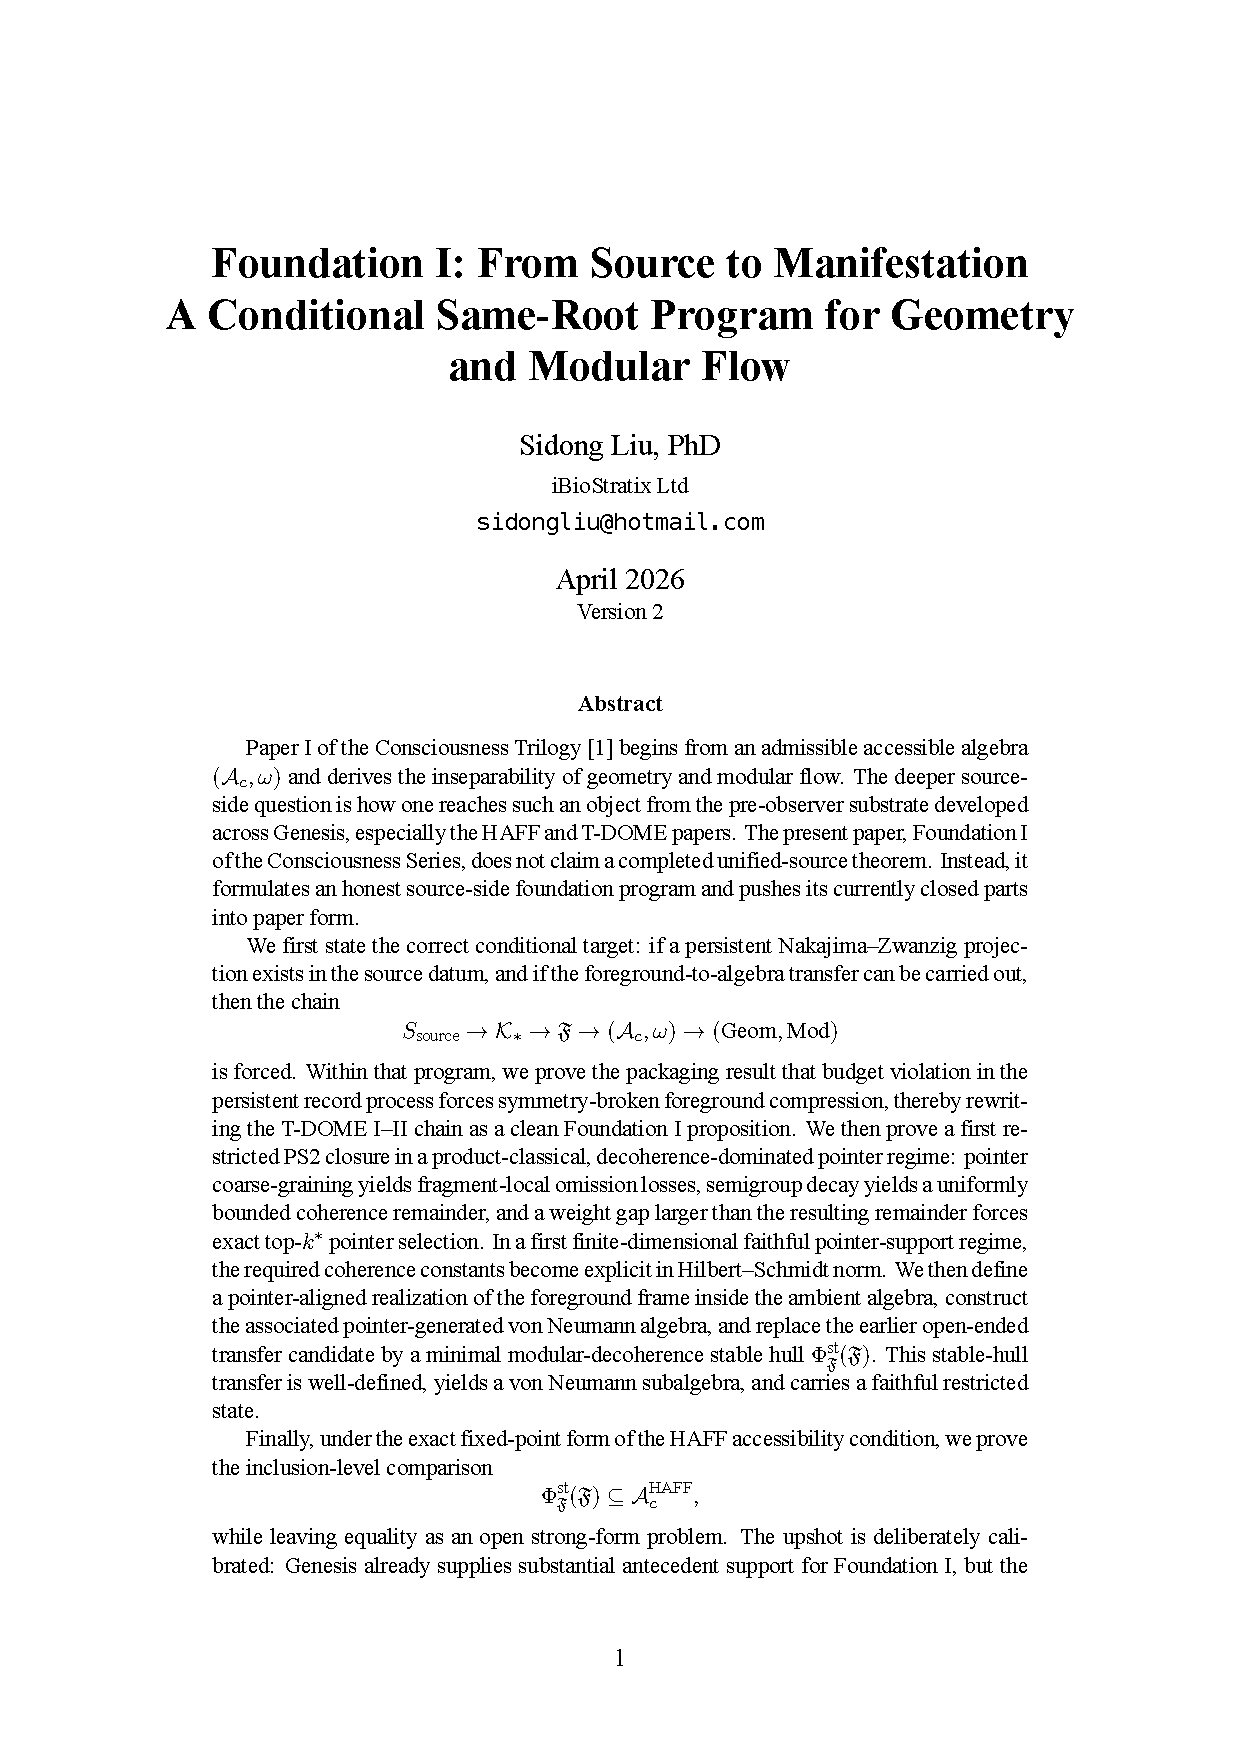
\includepdf[
  pages=-,
  pagecommand={\thispagestyle{empty}},
  addtotoc={1,chapter,1,{Foundation I: From Source to Manifestation},chap:foundationI}
]{../Zenodo/Foundation_I_From_Source_to_Manifestation_Zenodo_v2.pdf}

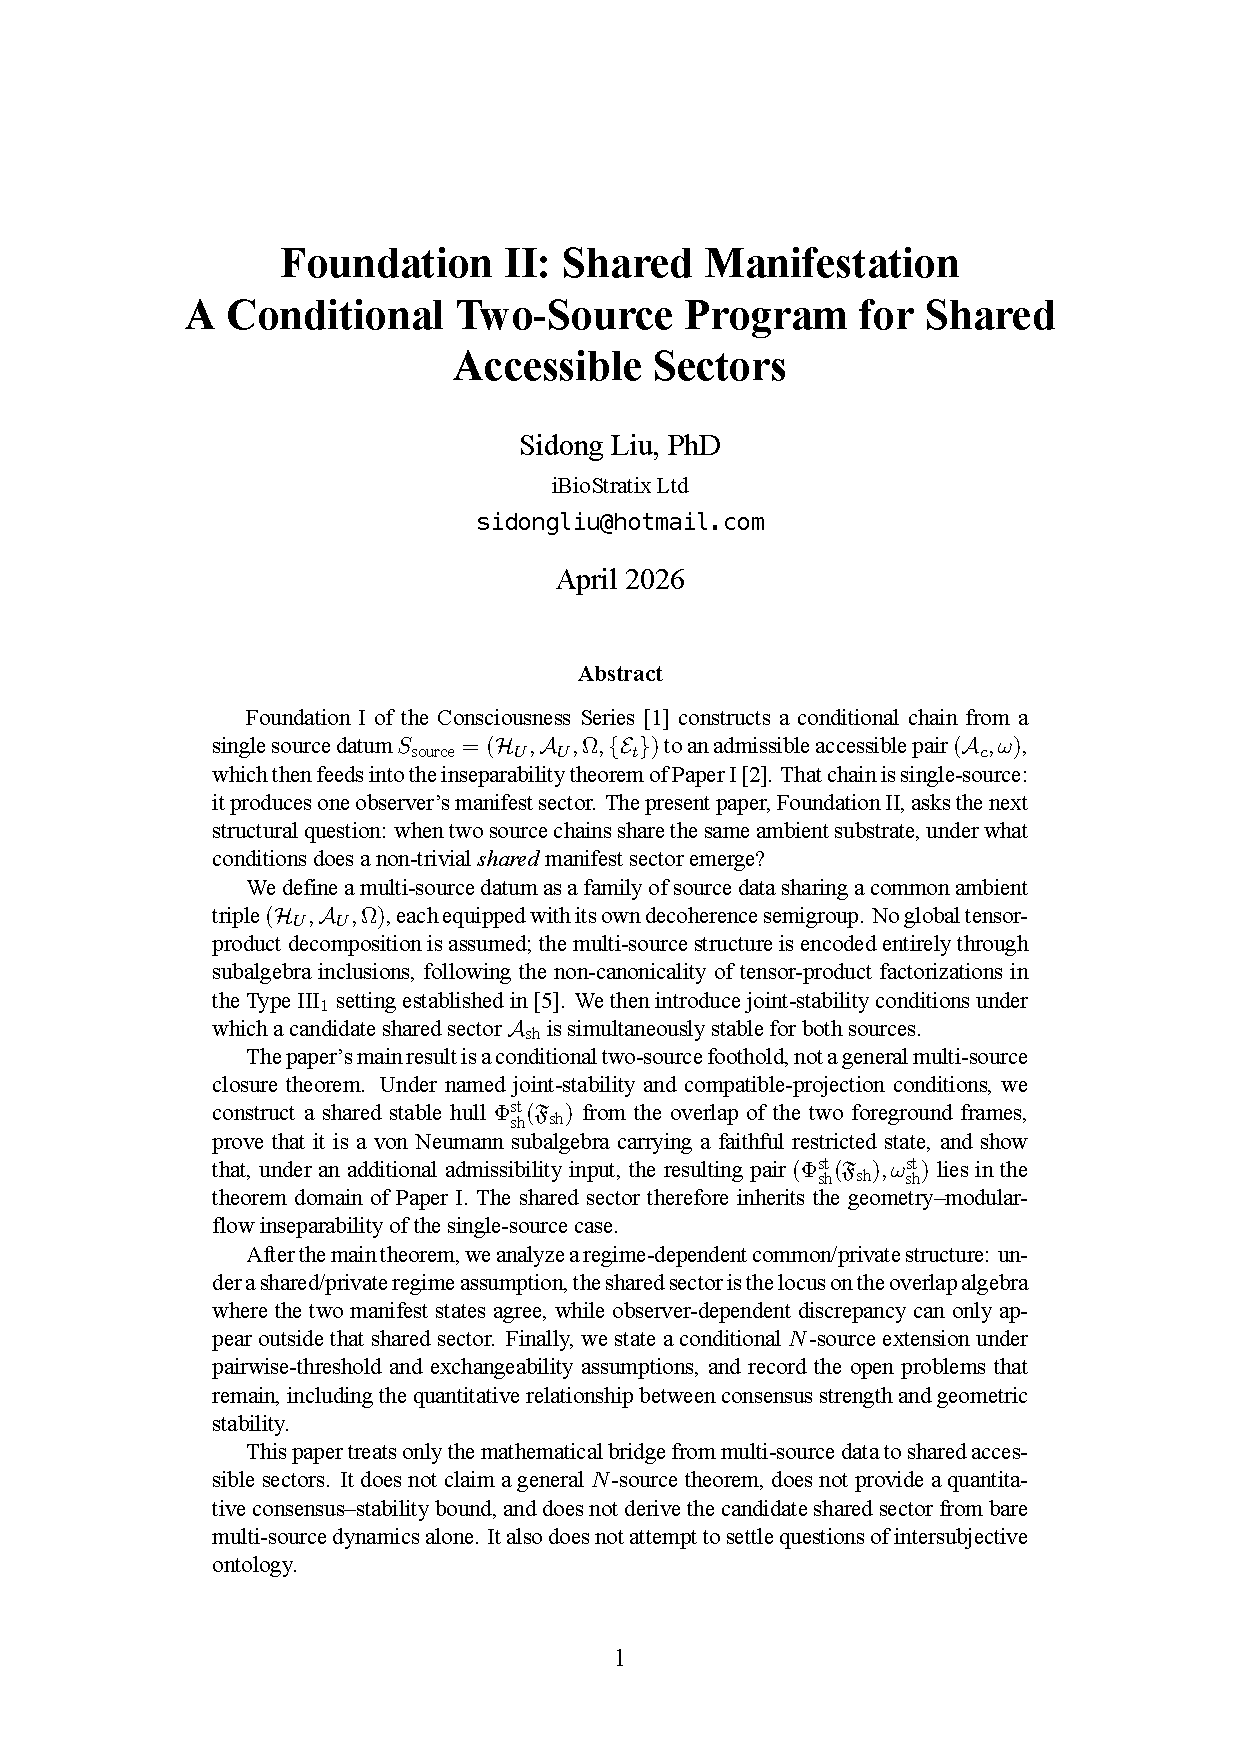
\includepdf[
  pages=-,
  pagecommand={\thispagestyle{empty}},
  addtotoc={1,chapter,1,{Foundation II: Shared Manifestation},chap:foundationII}
]{../Zenodo/Foundation_II_Shared_Manifestation_Zenodo.pdf}

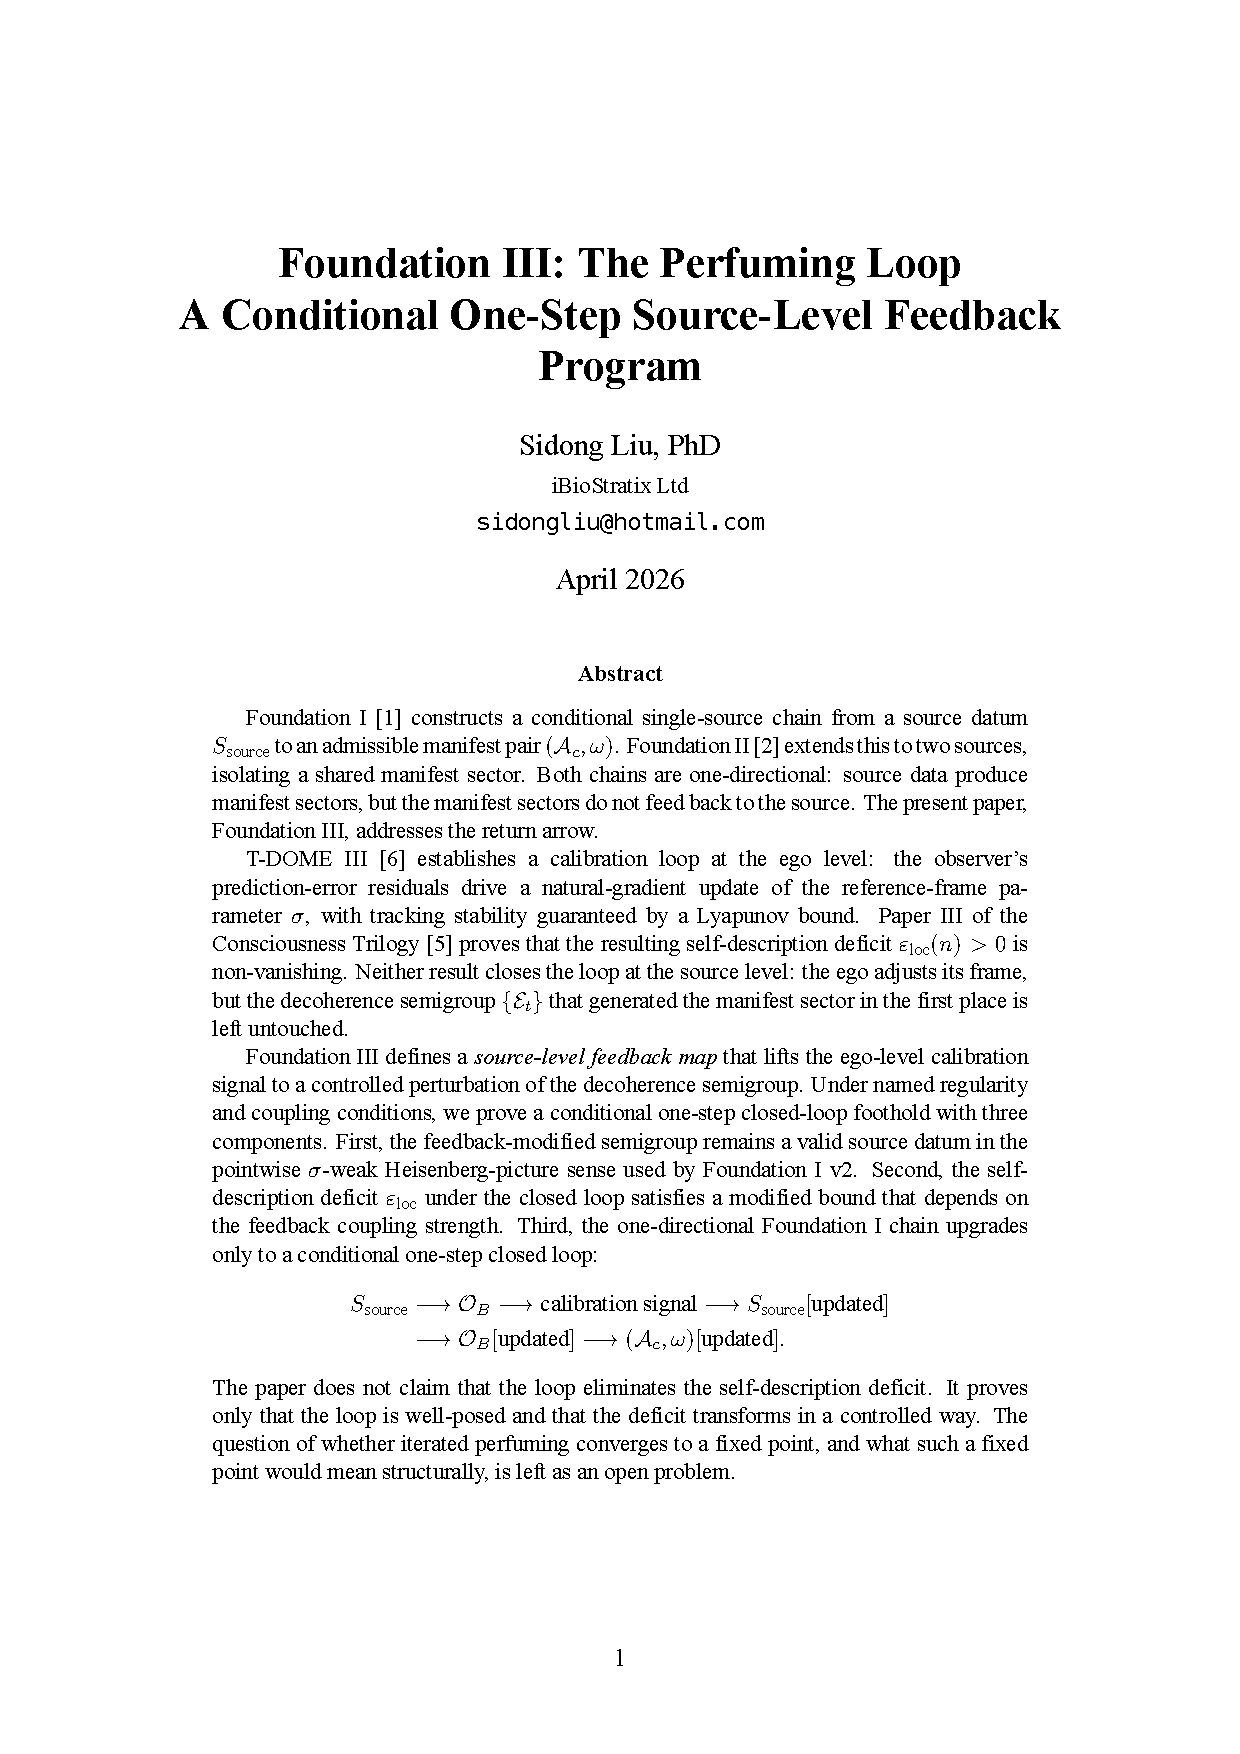
\includepdf[
  pages=-,
  pagecommand={\thispagestyle{empty}},
  addtotoc={1,chapter,1,{Foundation III: The Perfuming Loop},chap:foundationIII}
]{../Zenodo/Foundation_III_The_Perfuming_Loop_Zenodo.pdf}

\end{document}
